\chapter*{ВВЕДЕНИЕ}
\addcontentsline{toc}{chapter}{ВВЕДЕНИЕ}

В философском смысле сама жизнь -- это движение, то есть процесс.
Мы включены в разнообразные процессы: изменение уровня глюкозы в крови, появление солнечных пятен, рост цен акций и многие другие.
Независимо от того являемся ли мы их источником, участником или просто подвержены влиянию этих процессов,
нам требуются технологии наблюдения, анализа и прогнозирования явлений, описываемых большим объемом информации.

Задачи воспроизведения источника информации с целью анализа данных, поиска основных закономерностей и структур,
а также прогнозирования возможных будущих значений решается посредством использования временных рядов~\cite{myref1}.

Под временным рядом подразумевается последовательность наблюдений некоторого признака (случайной величины) x в
последовательные моменты времен~\cite{myref2}.
Элементы временного ряда включают в себя два обязательных параметра: отметку времени и значение показателя ряда,
соответствующее указанной отметке времени~\cite{myref9}.

Область применения временных рядов охватывает различные сферы: экономику~\cite{myref8, myref10, myref12, myref13}, биологию~\cite{myref11},
сейсмологию~\cite{myref14}, программирование~\cite{myref15} и так далее.

На рисунке~\ref{img1} представлен пример временного ряда цен на электроэнергию европейской территории РФ.

\begin{figure}[h]
    \centering
    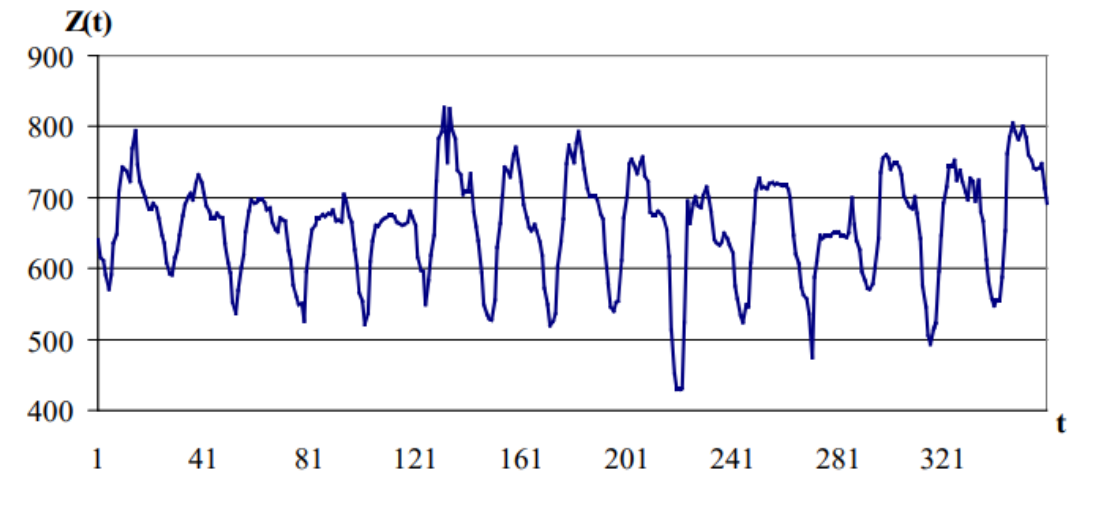
\includegraphics[height=0.2\textheight]{img/img1}
    \caption{Временной ряда цен на электроэнергию европейской территории РФ (в условных денежных единицах)~\cite{myref9}}
    \label{img1}
\end{figure}
\clearpage

Временные ряды дают возможность предугадать динамику отслеживаемых процессов.
Прогноз основывается на данных, которые фиксируются на протяжении некоторого времени, что требует организации их хранения.

В данной работе будут рассмотрены некоторые методы хранения и
прогнозирования временных рядов.
